\documentclass[letterpaper]{article}
\usepackage{amsmath}
\usepackage{amsfonts}
\usepackage{fontspec}
\usepackage{graphicx}
\usepackage{float}		%\begin{figure}[H] <- agrega el H
\usepackage{multirow}
\usepackage{multicol}
\usepackage{indentfirst}
\usepackage{caption} %comando \ContinuedFloat
\usepackage{array} %paquete para tabular
\usepackage{subcaption} %subfiguras y continuación de figura
\usepackage{pstricks-add}
\usepackage{bm}
\usepackage{enumitem} %cara utilizar distintos enumerate item


\newcolumntype{P}[1]{>{\centering\arraybackslash}p{#1}} % P{} (mayúscula) en vez de p{} (minúscula)
\newcommand{\vect}[1]{\boldsymbol{#1}} %notación vector \vect{•}
\renewcommand{\contentsname}{Índice}
\renewcommand{\figurename}{Figura}
\renewcommand{\tablename}{Tabla}
\renewcommand\refname{Referencias}

%%% quita los ":" del \caption
\makeatletter
\long\def\@makecaption#1#2{%
\vskip\abovecaptionskip
\sbox\@tempboxa{#1. #2}%
\ifdim \wd\@tempboxa >\hsize
#1. #2\par
\else
\global \@minipagefalse
\hb@xt@\hsize{\hfil\box\@tempboxa\hfil}%
\fi
\vskip\belowcaptionskip}
\makeatother
%%%%%%%%%%%%%%%%%%%%%%%%%


\pagestyle{plain}


%FORMATO PÁGINA
%\hoffset
\voffset=-2cm
\oddsidemargin=0.8cm
%\evensidemargin
%\topmargin 		%entre sup y encab
%\headheight		%tamaño encabezado
%\headsep			%sep encab y text
\textheight=23cm		%altura texto
\textwidth=15cm		%ancho texto
%\marginparsep	%sep notmargen y text
%\marginparwidth	%ancho nota al marg
\footskip=1cm		%pie de pag

\begin{document}

\thispagestyle{empty}

\hspace{-5mm}
\begin{minipage}[c]{7cm}
\centering

\includegraphics[width=4cm]{logoutfsm.jpg} \\
Universidad Técnica Federico Santa María
\end{minipage}
\hfill
\hspace{20mm}
\begin{minipage}[c]{7cm}
\centering

\includegraphics[width=4cm]{logomec1.jpg} \\
Departamento de Ingenieria Mecánica
\end{minipage}

\begin{center}
\vfill
 \Huge{{\bf Proyecto 1 }} \\ \vspace{1cm} 
 \Huge{Dinámica de fluidos computacional}
\vfill
\end{center}

\vfill \hfill
\begin{tabular}{l @{ : } l}
Nombre &   Ignacio Apablaza \\
Rol & 201141007-6  \\
Profesores & Romain Gers \\
			& Olivier Skurtys \\
Asignatura & IPM468 \\
\end{tabular}

\newpage
%---------------------------------------------


\tableofcontents


\newpage
%---------------------------------------------

\section{Resumen}






\newpage
%---------------------------------------------

\section{Introducción}







\newpage
%---------------------------------------------

\section{Metodología}

%---NOTA MENTAL PARA MI
\subsection{'para la preguntita 1'}
\begin{itemize}
\item hablar de fortran, programación orientada a objetos
\item hablar de la precision de la maquina
\item hablar de inestabilidad numerica
\item hablar de las series numericas (convergencia)
\item hablar de la serie fibbonacci
\item hablar de las subrutinas
\end{itemize}
%---FIN NOTA MENTAL
%---NOTA MENTAL PARA MI
\subsection{'para la preguntita 2'}
\begin{itemize}
\item hablar de euler implicito, familia esquema theta (crank nicolson), leapfrog, newmark
\item hablar de estabilidad espacio-tiempo (pasos de tiempo, dx,etc)
\item hablar de hablar de las arterias desde el punto de vista mec de fluidos
\item estimación del error
\item razon de convergencia de la malla (como afecta la malla en los resultados)
\item ...
\end{itemize}
%---FIN NOTA MENTAL
%---NOTA MENTAL PARA MI
\subsection{'para la preguntita 3'}
\begin{itemize}
\item LEER!!!
\end{itemize}
%---FIN NOTA MENTAL


Ecuación de onda

\begin{equation}
\dfrac{\partial^2 y}{\partial t^2} - \gamma \dfrac{\partial^2 y}{\partial x^2} = f
\end{equation} 

Esquema de discretización Newmark

\begin{equation}
v = \dfrac{\partial u}{\partial t}
\end{equation}

Luego, el desarrollo de Taylor de $v(t+ \Delta t) = t^{n+1}$ para un paso de tiempo $\Delta t$ es

\begin{equation}
v^{n+1} = v^{n} + \Delta t \dfrac{\partial v}{\partial t} (t= \xi)
\end{equation}

para $\xi \in [t,t+\Delta t]$ .como

\begin{equation}
\dfrac{\partial v}{partial t} = \dfrac{\partial^2 u}{\partial t^2} = \gamma \dfrac{\partial^2 u}{\partial x^2} + f 
\end{equation}

Reemplazando en la (ECUACION!) se tiene 




\newpage
%---------------------------------------------
\section{Desarrollo y Análisis}
%----
\subsection{Ejercicios en Fortran}
\subsubsection{Ejercicio 1}

Sea $A(n)$ un número real tal que
\begin{equation}
A(n) = \sum_{n=1}^\infty \dfrac{1}{n}
\end{equation}
Se implementa una programa en Fortran que permite calcular y graficar $A(n)$ para ciertos valores de $n$. En la Figura \ref{fig_P1_1_1} se grafica $A$ para simple y doble precisión. En la Figura \ref{fig_P1_1_2} Para doble y cuadruple precisión

\begin{figure} [H]
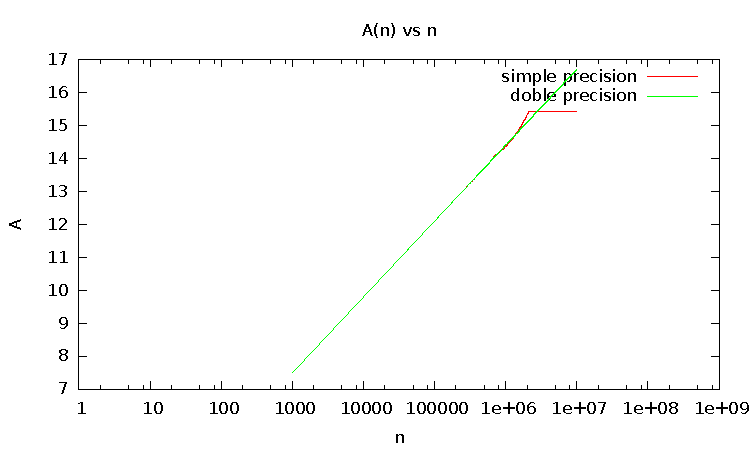
\includegraphics{./parte2/graficos/grafico_p1_1.pdf}
\caption{} \label{fig_P1_1_1}
\end{figure}

\begin{figure} [H]
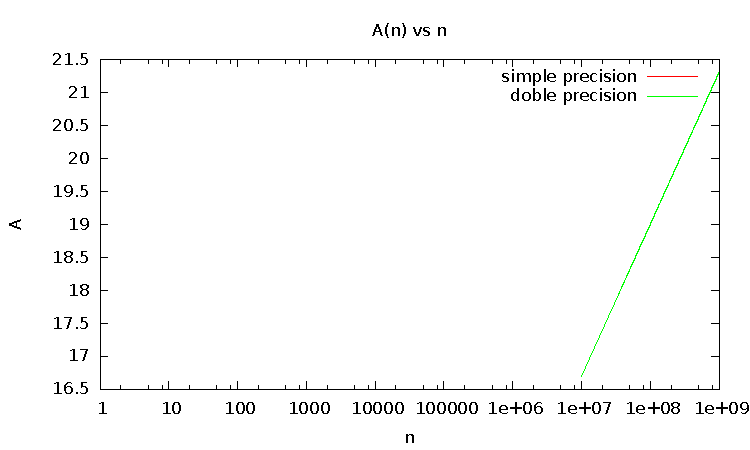
\includegraphics{./parte2/graficos/grafico_p1_2.pdf}
\caption{} \label{fig_P1_1_2}
\end{figure}

%----------------------------------------------
\subsubsection{Ejercicio 2}
Se implementa una rutina en Fortran que permite calcular los $n+1$ valores de la serie Fibonacci
\begin{equation}
u_{n+1} = u_{n} + u_{n-1} \hspace{1cm} \mbox{tal que} \hspace{0,5cm} u_0=0 \hspace{0,1cm} ; \hspace{0,1cm} u_1=1
\end{equation}
La serie se grafica para $n=100$

\begin{figure} [H]
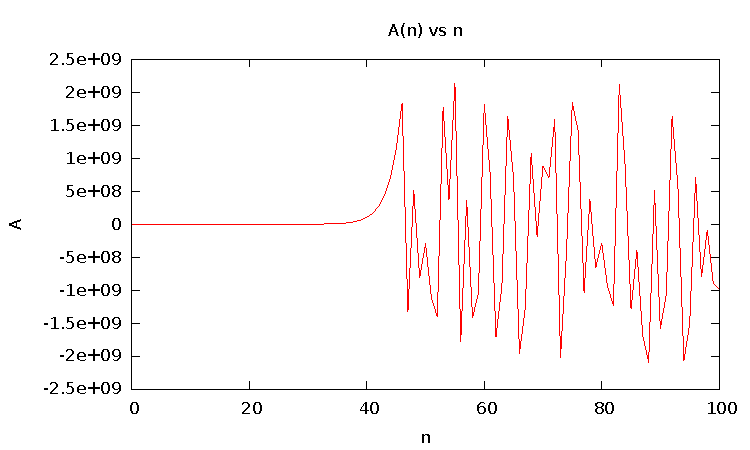
\includegraphics{./parte2/graficos/grafico_p2.pdf}
\caption{} \label{fig_P1_2}
\end{figure}
%----
\subsection{Estudio del comportamiento mecánico de una arteria}
%Estudio del comportamiento mecánico de una arteria

\subsection{Parte 1: Movimiento de una pared arterial}

Una arteria puede modelarse por un cilindro flexible de base circular, longitud $L$, radio $R_0$, cuyas paredes poseen un espesor $H$. Se supone que está constituido de un material elástico, incompresible, homogéneo e isotrópico. 

Un modelo simplificado que describe el comportamiento mecánico de la pared arterial en interacción con el flujo sanguíneo se obtiene considerando que el cilindro es constituido por un conjunto de anillos independientes uno de otros. De esta manera se puede despreciar las interacciones longitudinales y axiales a lo largo de la arteria. Luego, se supone que la arteria se deforma solamente en la dirección radial.

El radio de la arteria está dado por,

\begin{equation}
R(t) = R_0 + y(t)
\end{equation}

donde $y(t)$ es la deformación radial en función del tiempo $t$. Al aplicar la ley de Newton en el sistema de anillo independientes conduce a una ecuación que permite modelar el comportamiento mécanico de la pared de la arteria en función del tiempo,

\begin{equation} \label{PROBLEMA_PARTE2}
\dfrac{d^2 y(t)}{dt^2} + \beta \dfrac{dy(t)}{dt} + \alpha y(t) = \gamma (p(t)-p_0)
\end{equation}

donde,

\begin{equation}
\alpha = \dfrac{E}{\rho_w R^2_0} \hspace{0,5cm} \gamma = \dfrac{1}{\rho_w H} \hspace{0,5cm} \beta = \mbox{constante} > 0 
\end{equation}

Particularmente se modela la variación de la presión a lo largo de la arteria como una función sinusoidal que depende de la posición $x$ y el instante de tiempo $t$,

\begin{equation} \label{FUENTE_PARTE2}
(p-p_0) = x \Delta p  \left( a + b cos( \omega_0 t ) \right)
\end{equation} 

\subsubsection{Simulación 1}

Se calcula numericamente la ecuación \ref{PROBLEMA_PARTE2} con el término fuente \ref{FUENTE_PARTE2} y considerando los siguientes valores realistas para los parámetros físicos:
\begin{table}
\centering
\begin{tabular}{llll}
$L$		& = $5 \times 10 ^ {-2}$ m 				&	$b$	 		&= $133.32$ N m $^{-2}$ \\
$R_0$	& = $5 \times 10 ^ {-3}$ m 				&	$a$		 	&= $1333.2$ N m $^{-2}$ \\
$\rho_w$& = $1 \times 10 ^ {3}$ kg m $^{-3}$ 	&	$\Delta p$ 	&= $33.33$ N m $^{-2}$ \\
$H$		& = $3 \times 10 ^ {-4}$ m 				&	$w_0$ 		&= $2 \pi / 0.8$ \\
$E$		& = $9 \times 10 ^ {5}$ N m $^{-2}$ 	&				&
\end{tabular}
\caption{Parametros utilizados para la simulación 1} \label{PARAMETROS_PARTE2}
\end{table}

Y considerando a su vez dos parametros de $\beta$:
\begin{enumerate}[label=(\alph*)]
\item $\beta = \sqrt{ \alpha }$ 
\item $\beta = \alpha$
\end{enumerate}

Se reescribe la ecuación (\ref{PROBLEMA_PARTE2}) como un sustema de ecuaciones lineales. En forma matricial,

\begin{equation} \label{PROBLEMA_PARTE2_CORREGIDO}
\vec{y'}(t) = \vect{A} \vec{y} + \vec{b}
\end{equation}

donde $\vec{y} = \begin{vmatrix} y & y' \end{vmatrix}^T$ ($T$ significa transpuesta), y $\vec{b}(t)$ es un vector fuente dependiente del tiempo $t$. La matriz $\vect{A}$ resultante es,

\begin{equation}
\vect{A} = \begin{pmatrix}
0 & 1 \\ -\alpha & -\beta
\end{pmatrix}
\end{equation}

Se implementa una subrutina que permite calcular los valores propios de la matriz $\vect{A}$ de la ecuación \ref{PROBLEMA_PARTE2_CORREGIDO}. Utilizando los valores de la Tabla \ref{PARAMETROS_PARTE2} se obtiene:
\begin{enumerate} [label=(\alph*)]
\item $\beta = \sqrt{\alpha} = 6.0 \times 10^3 $
\begin{equation}
\vect{A} = \begin{pmatrix} 0 & 1 \\ 36.0 \times 10^6 & 6.0 \times 10^3 \end{pmatrix} \rightarrow 
\begin{matrix} \lambda_1 = & -3000.00 + 5196.15 i \\ \lambda_2 &= -3000.00 - 5196.15 i \end{matrix}
\end{equation} 
\item $\beta = \alpha =  36.0 \times 10^6 $
\begin{equation}
\vect{A} = \begin{pmatrix} 0 & 1 \\ 36.0 \times 10^6 & 6.0 \times 10^3 \end{pmatrix} \rightarrow 
\begin{matrix} \lambda_1 = & -3000.00 + 5196.15 i \\ \lambda_2 &= -3000.00 - 5196.15 i \end{matrix}
\end{equation} 
\end{enumerate}

Se implementa una subrutina que permite calcular la ecuacion (AGREGAR ECUACION) usando el método de Euler Implícito para dos valores de $\beta$ 



%------------------------------------

HABLAR DE LOS VALORES PROPIOS

%------------------------------------

Discretizacion de la ecuación por el método Euler Implicito
\begin{align}
\dfrac{y^n - y^{n-1}}{\Delta t} &= z^n \\
\dfrac{z^n - z^{n-1}}{\Delta t} &= -\alpha y^n - \beta z^n + \gamma (p_n-p_0) \\
\end{align}

Reordenando los valores en los pasos de tiempo $n$ $n-1$ en el lado izquierdo y derecho respectivamente, se expresa la relacion (ECUACION ANTERIOR) en forma matricial como,
\begin{equation}
\vect{A} \cdot \begin{Bmatrix}
y^n \\ z^n
\end{Bmatrix} =
\begin{Bmatrix}
y^{n-1} \\ z^{n-1}
\end{Bmatrix} +
\Delta t \begin{Bmatrix}
0 \\ \gamma (p_n-p_0)
\end{Bmatrix}
\end{equation}
donde
\begin{equation}
\vect{A} = \begin{pmatrix}
1 & -\Delta t \\
\Delta t \alpha & 1+ \Delta t \beta
\end{pmatrix}
\end{equation}


Despenjando las incognitas se obtiene,
\begin{equation}
\begin{Bmatrix}
y^n \\ z^n
\end{Bmatrix} =
\vect{A}^{-1} \cdot \begin{Bmatrix}
y^{n-1} \\ z^{n-1}
\end{Bmatrix} +
\Delta t \vect{A}^{-1} \cdot  \begin{Bmatrix}
0 \\ \gamma (p_n-p_0)
\end{Bmatrix}
\end{equation}
donde
\begin{equation}
\vect{A}^{-1} = 
\dfrac{1}{1 + \beta \Delta t + \alpha (\Delta t) ^ 2}
\begin{pmatrix}
1+\beta \Delta t & \Delta t \\
-\Delta t \alpha & 1 
\end{pmatrix}
\end{equation}

%------------------------

Discretizacion de la ecuación por el método Crank Nicolson

\begin{align}
\dfrac{y^{n+1}-y^n}{\Delta t} & = \dfrac{1}{2} \left( z^{n+1} + z^n \right) \\
\dfrac{z^{n+1}-z^n}{\Delta t} &= \dfrac{1}{2} \left( -\alpha y^{n+1} - \beta y^{n+1} + \gamma (p_{n+1}-p_0) \right) + \dfrac{1}{2} \left( -\alpha y^{n} - \beta y^{n} + \gamma (p_{n}-p_0) \right)  
\end{align}

Reordenando los valores en los pasos de tiempo $n$ $n-1$ en el lado izquierdo y derecho respectivamente, se expresa la relacion (ECUACION ANTERIOR) en forma matricial como,

\begin{equation}
\vect{A} \cdot
\begin{Bmatrix}
y^{n+1} \\ z^{n+1}
\end{Bmatrix} =
\vect{B} \cdot
\begin{Bmatrix}
y^n \\ z^n
\end{Bmatrix} + \dfrac{\Delta t}{2}
\begin{Bmatrix}
0 \\ \left( \gamma (p_{n+1}-p_0) + \gamma (p_{n}-p_0) \right)
\end{Bmatrix}
\end{equation}

donde
\begin{equation}
\vect{A} = \begin{pmatrix}
1 & -\dfrac{\Delta t}{2} \\
\dfrac{\alpha \Delta t}{2} & 1+ \dfrac{\beta \Delta t}{2}
\end{pmatrix} 
\end{equation}

\begin{equation}
\vect{B} = \begin{pmatrix}
1 & \dfrac{\Delta t}{2} \\
-\dfrac{\alpha \Delta t}{2} & 1-\dfrac{\beta \Delta t}{2}
\end{pmatrix}
\end{equation}

Despejando las variables incognitas se obtiene,

\begin{equation}
\begin{Bmatrix}
y^{n+1} \\ z^{n+1} 
\end{Bmatrix} =
\vect{A}^{n-1} \cdot \vect{B} \cdot 
\begin{Bmatrix}
y^n \\ z^n 
\end{Bmatrix} + \dfrac{\Delta t}{2} \vect{A}^{-1} \cdot
\begin{Bmatrix}
0 \\ \left( \gamma (p_{n+1}-p_0) + \gamma (p_{n}-p_0) \right)
\end{Bmatrix}
\end{equation}

donde 
\begin{equation}
\vect{A}^{-1} = \dfrac{1}{1 + \beta \dfrac{\Delta t}{2} + \alpha \left( \dfrac{\Delta t}{2} \right)^2 } 
\begin{pmatrix}
1 + \dfrac{\beta \Delta t}{2} & \dfrac{\Delta t}{2}\\
-\dfrac{\alpha \Delta t}{2} & 1 
\end{pmatrix}
\end{equation}

%-----------------------
\subsection{Parte 2: Un modelo hiperbólico para la interacción de la sangre con la pared}

\begin{equation}
\dfrac{\partial^2 u}{\partial t^2} - \gamma^2 \dfrac{\partial^2 u}{\partial x^2} = f \hspace{0,5cm} x \in ] \alpha , \beta [
\end{equation}

Esquema de discretización de Leapfrog
\begin{equation}
u^{n+1}_j - 2u^n_j + u^{n-1} = (\gamma \lambda)^2 ( u^n_{j-1} -2 u^n_j + u^n_{j+1} ) + f^n_j
\end{equation}
donde $\lambda=\dfrac{\Delta t}{\Delta x}$

%----
\subsection{Atractor de Lorenz}
%ATRACTOR DE LORENZ
El sistema de ecuaciones de Lorenz es un ejemplo de un sistema de ecuaciones diferenciales de orden 1, tridimensional, no lineal, que tiene un comportamiento caótico para algunos valores de sus parámetros. Este sistema de ecuaciones permite modelar los rollos de convección que se producen en la atmosfera terrestre. Es un modelo simplificado de la convección de Rayleigh-Benard (ecuaciones de Navier-Stokes con hipótesis de Boussinesq).
\begin{equation}
\left\{ 
\begin{matrix}
dx/dt =& Pr (y(t) - x(yt)) \\
dy/dt =& Ra x(t) - y(t) - x(t)z(t) \\
dz/dt =& x(t) y(t) - \beta z(t)
\end{matrix} \right.
\end{equation}
Donde $Pr$ es el número de Prandtl y $Ra$ es el número de Rayleigh. Las variables dinámicas $x$, $y$ y $z$ represetan el estado del sistema a cada instante $t$:

\begin{itemize}
\item x(t) es proporcional a la intensidad del movimiento de convección  
\item y(t) es proporcional a la diferencia de temperatura entre las corrientes ascendentes y descendentes
\item z(t) es proporcional a la diferencia entre el perfil vertical de temperatura y un perfil vertical de temperatura lineal
\end{itemize}

Los sistemas dinámicos son sistemas que son función del tiempo. Que sea caótico significa que varia de manera no lineal y a su vez que el sistema presenta sensibilidad a frente a los parámetros entrada. Además presentan un comportamiento oscilante, pudiendo ser periodico o no periodico. \\

\subsubsection{Parte 1}
Las Figuras \ref{lorenz1} y \ref{lorenz2} reproducen los gráficos del articulo \textit{Deterministic Nonperiodic Flow} de Lorenz
\begin{figure} [H]
\begin{center}
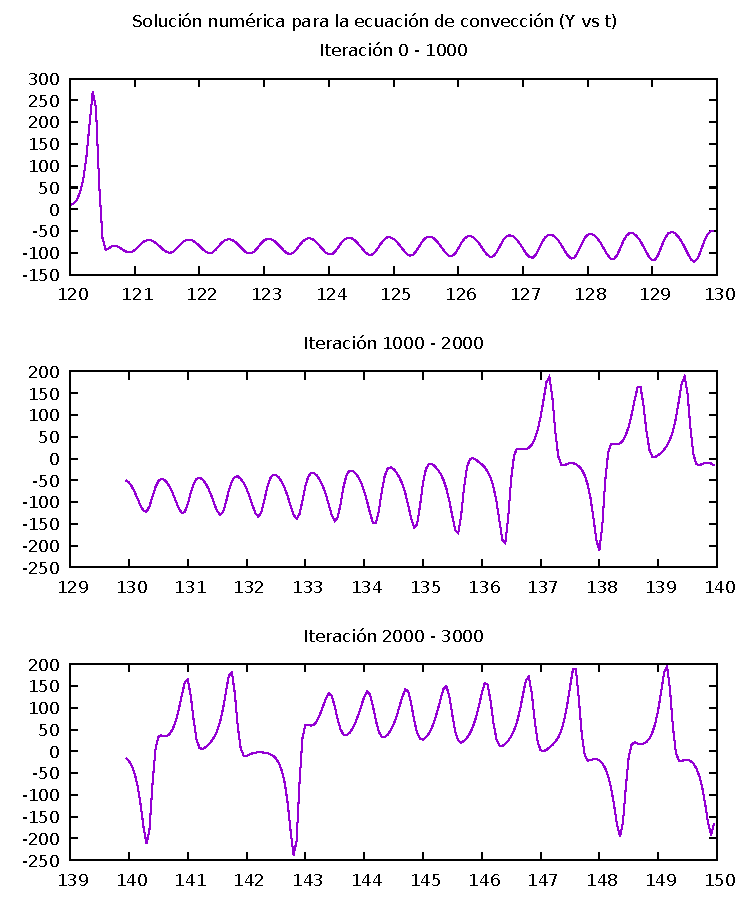
\includegraphics[width=0.8\textwidth]{./parte4/graficos/FIGURA1.pdf}
\caption{} \label{lorenz1}
\end{center}
\end{figure}

\begin{figure} [H]
\begin{center}
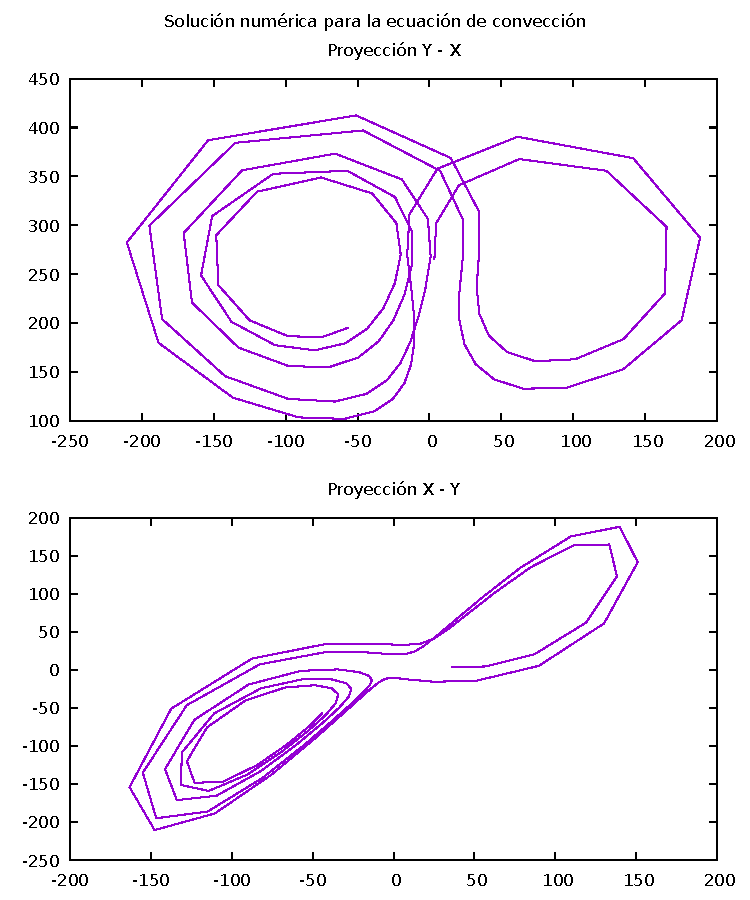
\includegraphics[width=0.8\textwidth]{./parte4/graficos/FIGURA2.pdf}
\caption{} \label{lorenz2}
\end{center}
\end{figure}

%---------------------------

\subsubsection{Parte 2}

Se grafica la solución a la ecuación de convección utilizando los siguientes valores: $Pr=10$, $\beta= 8/3$ y $Ra = 0.5 \, , \, 10 , \, 28$ 

\begin{figure} [H]
\begin{center}
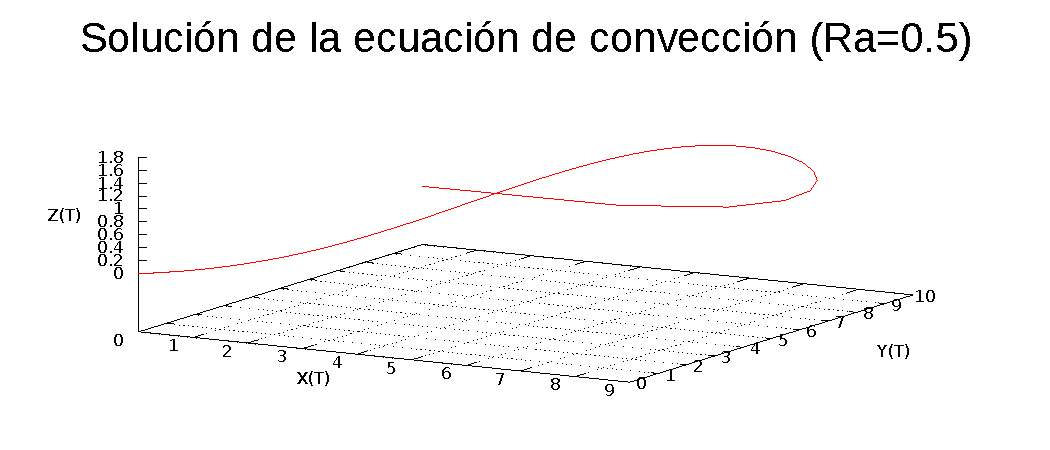
\includegraphics[width=0.8\textwidth]{./parte4/graficos/grafico_P3_3d_ra05.pdf}
\caption{}
\end{center}
\end{figure}

\begin{figure} [H]
\begin{center}
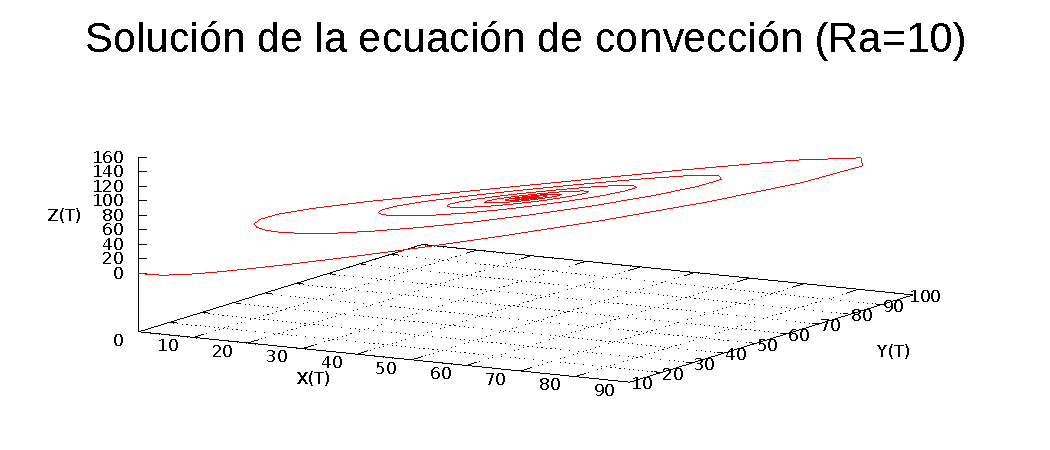
\includegraphics[width=0.8\textwidth]{./parte4/graficos/grafico_P3_3d_ra10.pdf}
\caption{}
\end{center}
\end{figure}

\begin{figure} [H]
\begin{center}
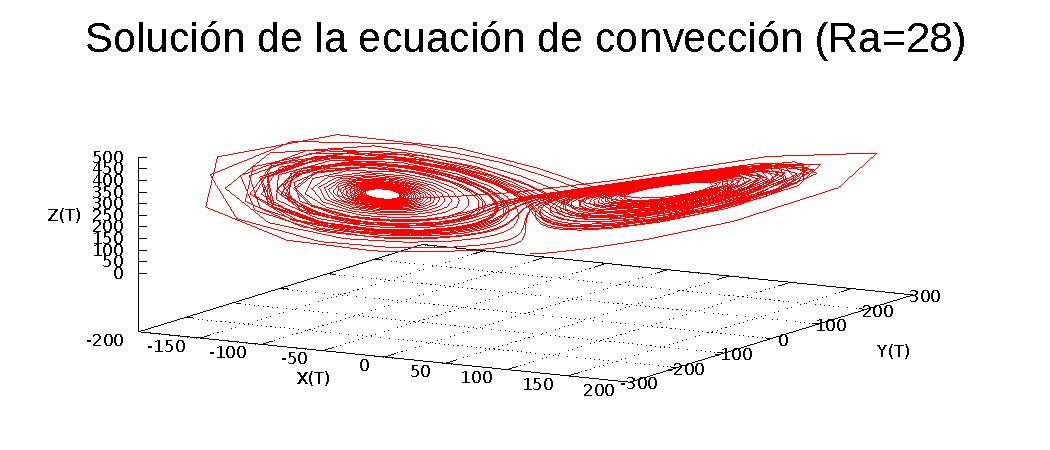
\includegraphics[width=0.8\textwidth]{./parte4/graficos/grafico_P3_3d_ra28.pdf}
\caption{}
\end{center}
\end{figure}

%---------------------------

\subsubsection{Parte 3}
Haciendo variar paulatinamente $Ra$ entre 0 y 30

\begin{figure} [H]
\hspace{-1cm} 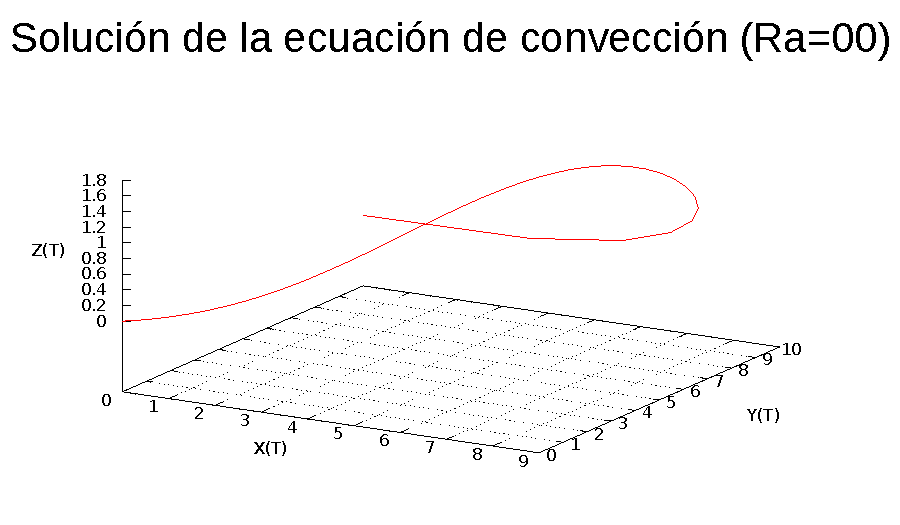
\includegraphics[width=0.6\textwidth]{./parte4/graficos/grafico_P3_3d_ra00.pdf}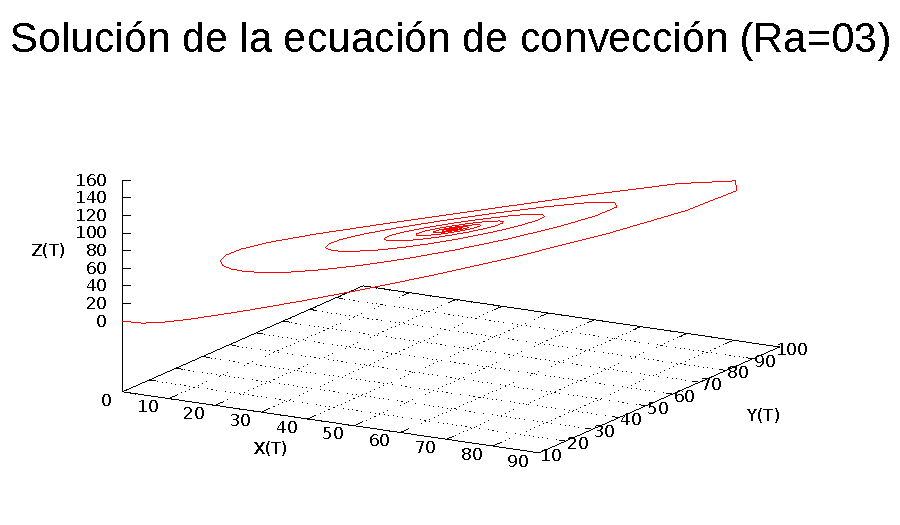
\includegraphics[width=0.6\textwidth]{./parte4/graficos/grafico_P3_3d_ra03.pdf}
\caption{} 
\end{figure}

\begin{figure} [H]
\hspace{-1cm} 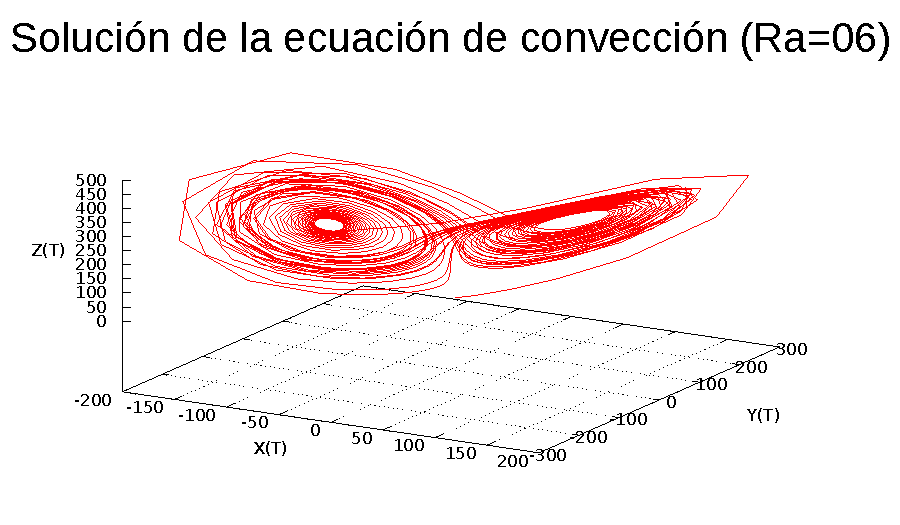
\includegraphics[width=0.6\textwidth]{./parte4/graficos/grafico_P3_3d_ra06.pdf}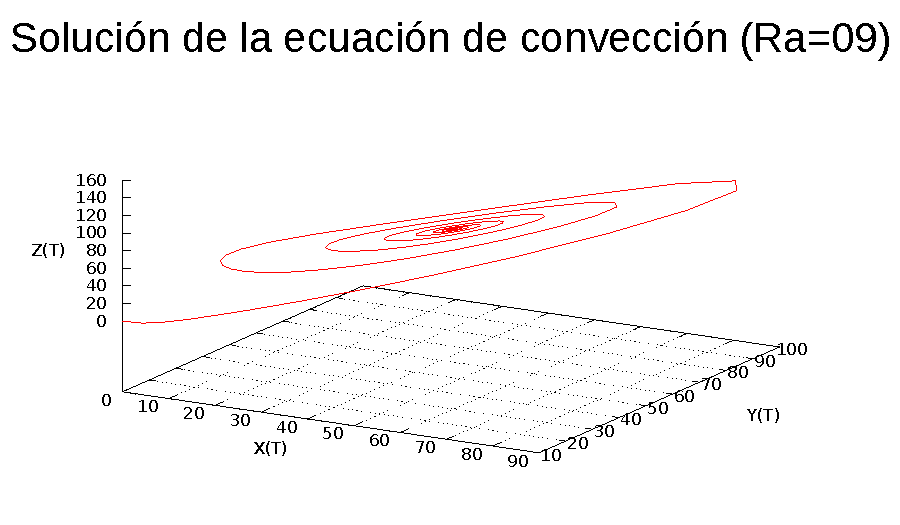
\includegraphics[width=0.6\textwidth]{./parte4/graficos/grafico_P3_3d_ra09.pdf}
\caption{} 
\end{figure}

\begin{figure} [H]
\hspace{-1cm} 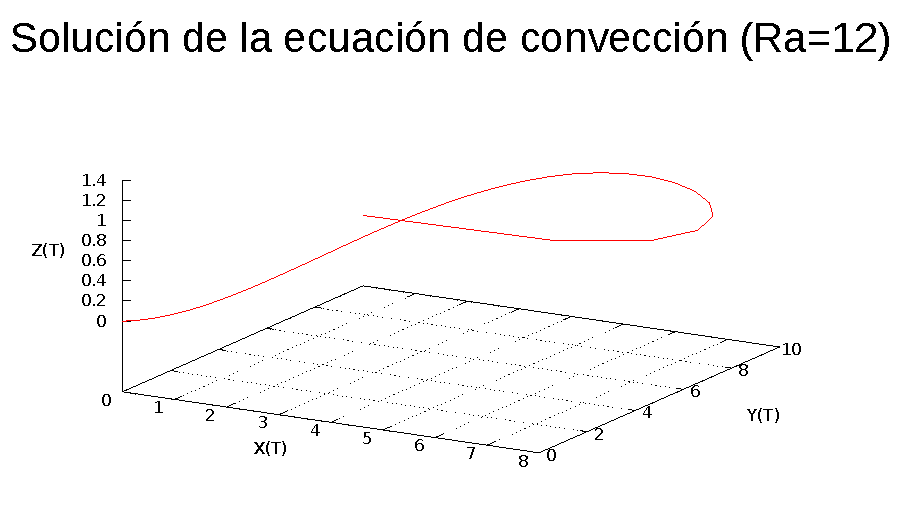
\includegraphics[width=0.6\textwidth]{./parte4/graficos/grafico_P3_3d_ra12.pdf}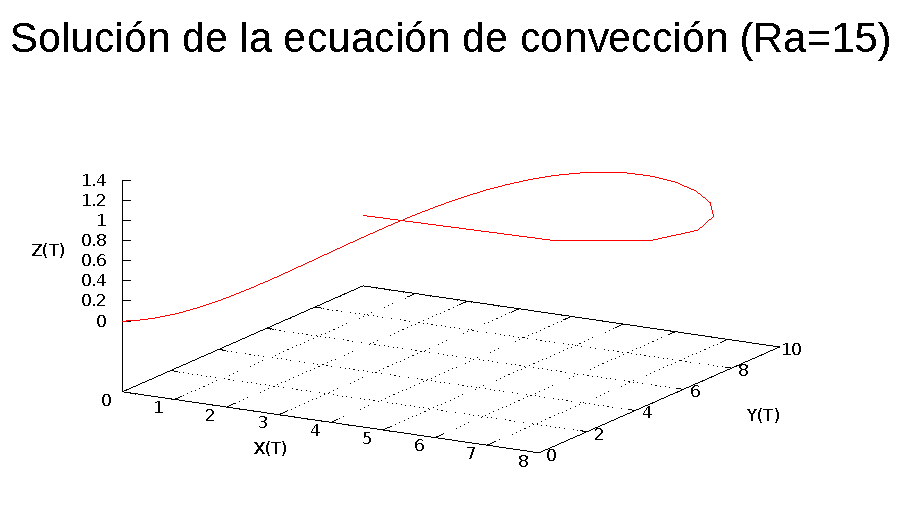
\includegraphics[width=0.6\textwidth]{./parte4/graficos/grafico_P3_3d_ra15.pdf}
\caption{} 
\end{figure}

\begin{figure} [H]
\hspace{-1cm} 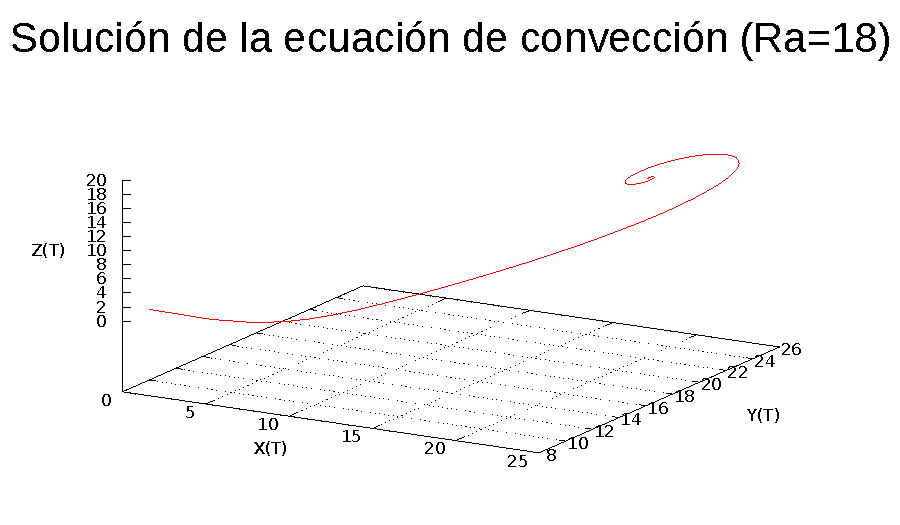
\includegraphics[width=0.6\textwidth]{./parte4/graficos/grafico_P3_3d_ra18.pdf}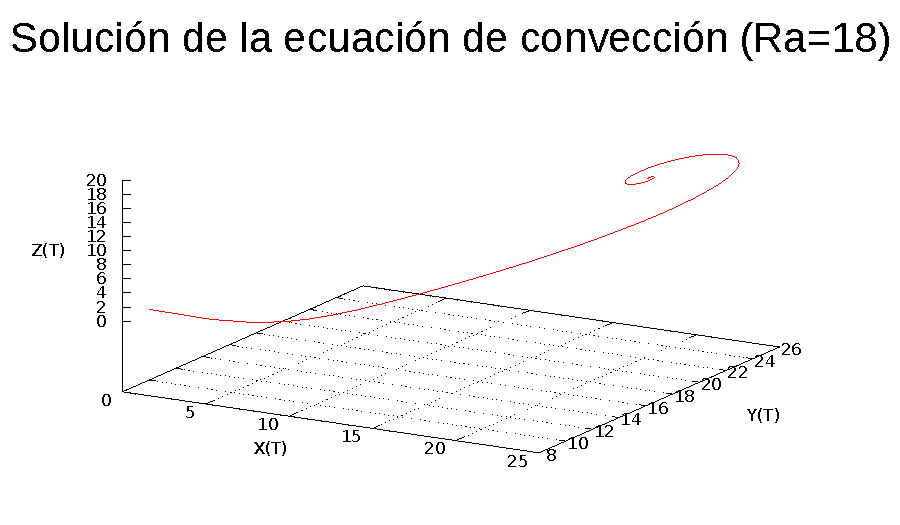
\includegraphics[width=0.6\textwidth]{./parte4/graficos/grafico_P3_3d_ra18.pdf}
\caption{} 
\end{figure}

\begin{figure} [H]
\hspace{-1cm} 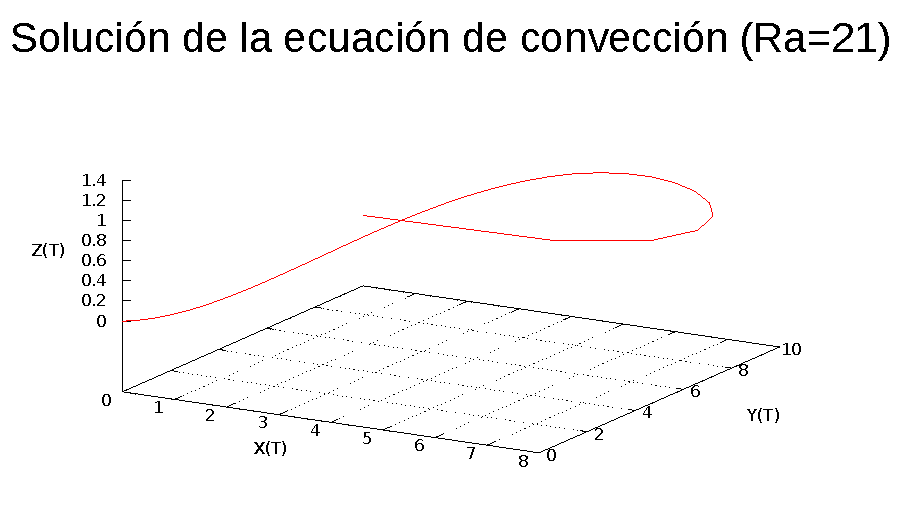
\includegraphics[width=0.6\textwidth]{./parte4/graficos/grafico_P3_3d_ra21.pdf}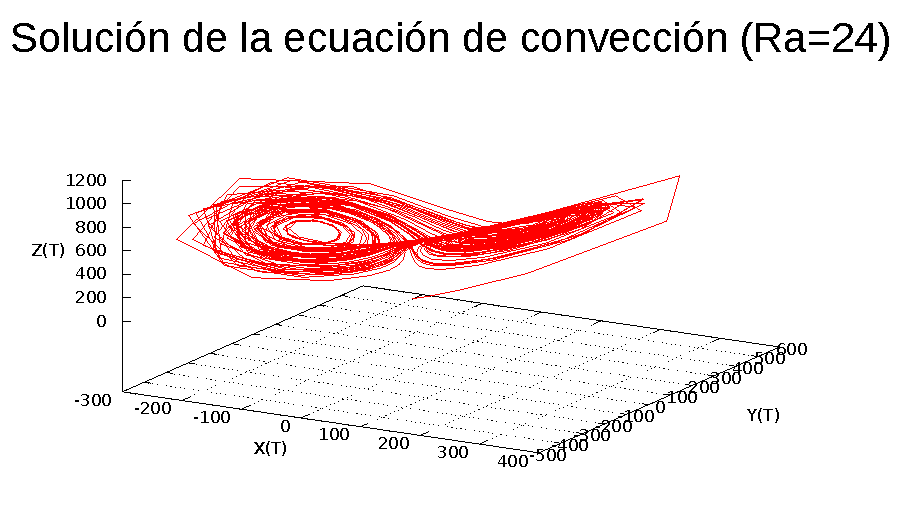
\includegraphics[width=0.6\textwidth]{./parte4/graficos/grafico_P3_3d_ra24.pdf}
\caption{} 
\end{figure}

\begin{figure} [H]
\hspace{-1cm} 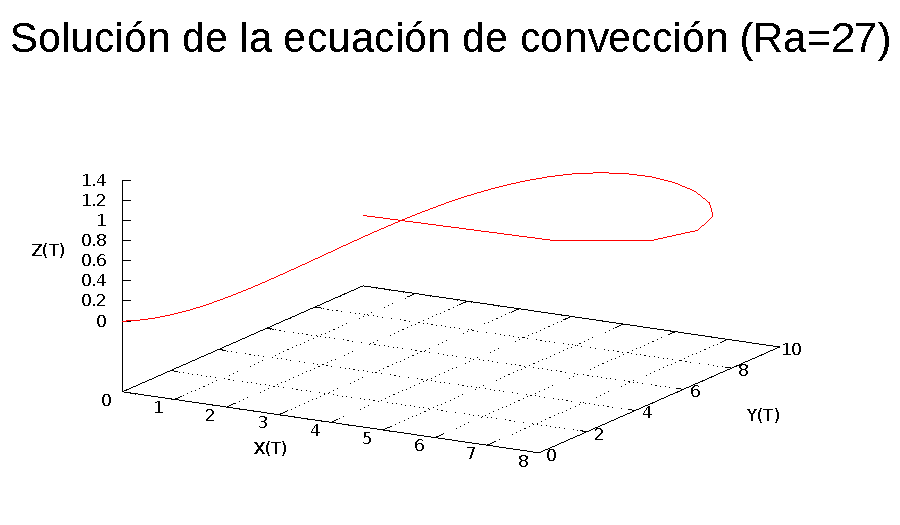
\includegraphics[width=0.6\textwidth]{./parte4/graficos/grafico_P3_3d_ra27.pdf}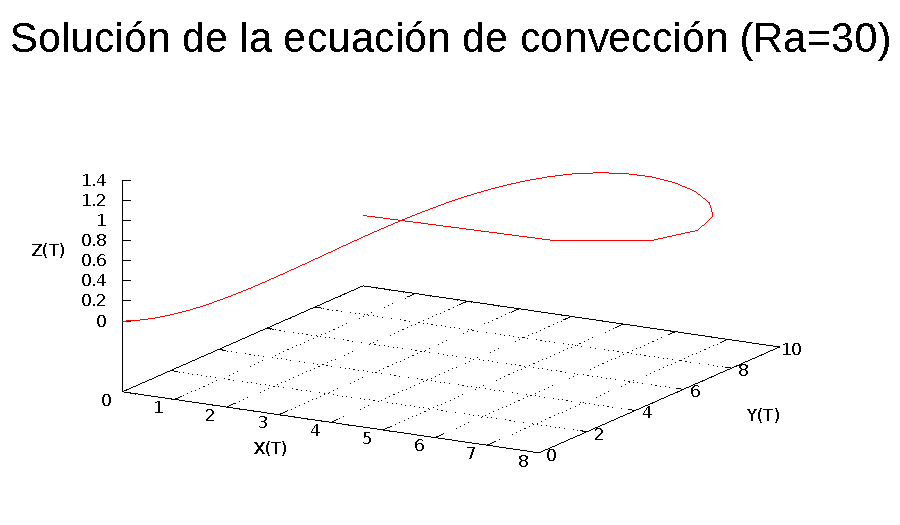
\includegraphics[width=0.6\textwidth]{./parte4/graficos/grafico_P3_3d_ra30.pdf}
\caption{} 
\end{figure}

\newpage
%---------------------------------------------
\section{Conclusiones y Observaciones}

\newpage
%---------------------------------------------

\begin{thebibliography}{3}
\bibitem{belytschko} \textsc{Dolbow, J., Belytschko, T.,} \textit{An Introduction to Programming the Meshless Element Free Garlekin Method},Archives of Computational Methods in Engineering vol. 5, 3, 207-241 (1998)

\bibitem{liu} \textsc{G.R. Liu} y \textsc{Y.T. Gu}, \textit{An Introduction to Meshfree Methods and Their Programming},
Editorial Springer, 2005, capítulos 1-3 y 6, ISBN-10 1-4020-3228-5

\bibitem{liu2} \textsc{G.R. Liu}, \textit{Meshfree Methods: Moving Beyond The Finite Element Method}, 2da edición,
Editorial CRC Press, 2010, capítulos 1 y 2, ISBN 978-1-4200-8209-8
\end{thebibliography}

\end{document}
